\documentclass[
%%dvips
%%,draft
10pt]{beamer}
%\hypersetup{pdfpagemode=FullScreen}

\mode<presentation>
{
  \usetheme{Warsaw}
  \usecolortheme{seahorse}
%  \usecolortheme{beetle}

  % or ...

  \setbeamercovered{transparent}
  % or whatever (possibly just delete it)
}
\usepackage[english]{babel}
% or whatever

\usepackage[latin1]{inputenc}
% or whatever

%Create a version that uses the handout overlay specifications.  You might wish to choose a different color and/or presentation theme for the handout.  When printing a handout created this way, you will typically wish to print at least two and possibly four slides on each page. The easiest way of doing so is presumably to use pgfpages as follows:
%\documentclass[handout]{beamer}
%\usepackage{pgfpages}
%\pgfpagesuselayout{4 on 1}[letterpaper,border shrink=5mm]


\usepackage{times}
\usepackage{url}
\usepackage{graphicx}
\usepackage[T1]{fontenc}
\usepackage{amsmath}
\usepackage{subfigure}
\usepackage{overpic}
\usepackage{xcolor}
\newcommand{\myitem}{\vskip3mm \item}
\newcommand{\given}{\,|\,}

% Or whatever. Note that the encoding and the font should match. If T1
% does not look nice, try deleting the line with the fontenc.

\newcommand{\argmax}{\operatornamewithlimits{argmax}}

\newcommand{\var}{\mbox{var}}
\newcommand{\Var}{\mbox{var}}
\newcommand{\corr}{\mbox{Corr}}
\newcommand{\Corr}{\mbox{Corr}}
\newcommand{\cor}{\mbox{Corr}}
\newcommand{\Cor}{\mbox{Corr}}
\newcommand{\cov}{\mbox{Cov}}
\newcommand{\Cov}{\mbox{Cov}}
\newcommand{\AR}{\mbox{AR}}
\newcommand{\CS}{\mbox{CS}}
\newcommand{\sd}{\mbox{sd}}
\newcommand{\SD}{\mbox{sd}}
\newcommand{\ANTE}{\mbox{ANTE}}
\newcommand{\UN}{\mbox{UN}}
\newcommand{\betadist}{\mbox{Beta}}


\definecolorset{rgb}{}{}{darkred,0.8,0,0;darkgreen,0,0.5,0;darkblue,0,0,0.5}

\usepackage{bm}
\renewcommand{\vec}[1]{
        \ensuremath{
                \bm{\mathrm{#1}}
        }
}

\usepackage{color}
\usepackage{ulem}
\usepackage{wrapfig}
\newcommand{\fder}[1]{\frac{d}{d #1}}
\newcommand{\hder}[2]{\frac{d^{#2}}{d {#1}^{#2}}}
\newcommand{\fpart}[1]{\frac{\partial}{\partial #1}}
\newcommand{\hpart}[2]{\frac{\partial^{#2}}{\partial {#1}^{#2}}}



%\newcommand{\data}{\vec{Y}}


%\newcommand{\parent}[1]{_{\mbox{\tiny pa}(#1)}}
%\renewcommand{\root}{_{\mbox{\tiny root}}}

%\usepackage{movie15}

\title[BIOSTAT 241]{Spatial Data Science and BIG DATA Analytics for Geographic Information Sciences}
%\subtitle{Grad School in Biostatistics at UCLA} % (optional)

\author[Sudipto~Banerjee]{Sudipto~Banerjee}

\institute[UCLA] % (optional, but mostly needed)
{
  Professor and Chair of Biostatistics \\
  Professor of Statistics \\
  Affiliate Member, Institute of the Environment \& Sustainability\\
  University of California Los Angeles (UCLA)\\
  sudipto@ucla.edu \\
%
% - Use the \inst command only if there are several affiliations.
% - Keep it simple, no one is interested in your street address.
}
\date[Spring, 2021]{Spring, 2021}

\subject{}
% This is only inserted into the PDF information catalog. Can be left
% out.

% Delete this, if you do not want the table of contents to pop up at
% the beginning of each subsection:
%\AtBeginSubsection[]
%{
%  \begin{frame}<beamer>
%    \frametitle{Outline}
%    \tableofcontents[currentsection,currentsubsection]
%  \end{frame}
%}


% If you wish to uncover everything in a step-wise fashion, uncomment
% the following command:

%\beamerdefaultoverlayspecification{<+->}


\begin{document}

\begin{frame}

  \titlepage

%\begin{center}
  
\includegraphics[height=.5in]{figs/FSPH_logo.jpg}\\
%\end{center}

\end{frame}


\begin{frame}{SIT: Spatial Information Technologies}
 
\begin{center}
 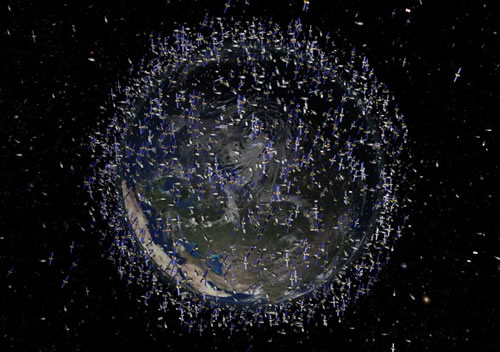
\includegraphics[width=\textwidth]{figs/space-debris.jpg}
\end{center}
 
\end{frame}


\begin{frame}{SIT: Spatial Information Technologies}
 
 \begin{center}
  Some neighbourhoods in Kolkata
  
  \medskip
  
  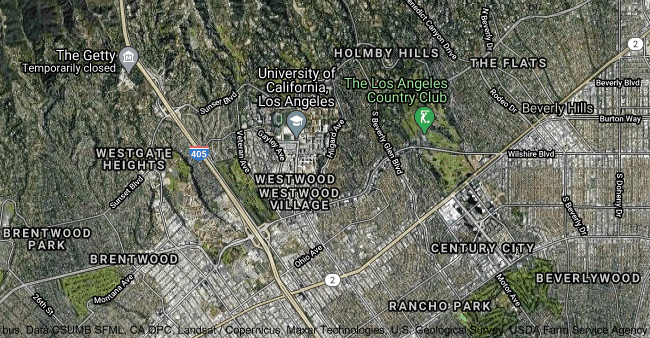
\includegraphics[scale=0.45]{figs/Westwood_Satellite_Map.png}
 \end{center}
 
\end{frame}

\begin{frame}{Geographic Information Systems (GIS)}
 
 \begin{center}
  Creating Databases for Maps
  
  \medskip
  
  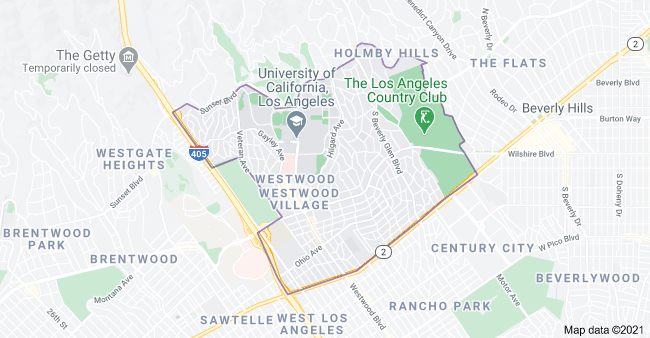
\includegraphics[scale=0.45]{figs/Westwood_GIS_Map.png}
 \end{center}
 
\end{frame}


\begin{frame}{Global Positioning Systems (GPS)}
 
\begin{center}
 A wearable GPS device 
 
 \medskip

 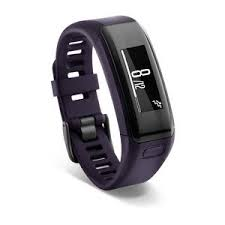
\includegraphics[width=0.5\textwidth]{figs/WearableGPS.jpg}
\end{center}
 
\end{frame}

\begin{frame}{Monitors for Physical Activity}
 
 \begin{itemize}\setlength{\itemsep}{0.4cm}
  \item Small motion sensor detectors (accelerometers) have generated substantial interest in monitoring human activity.
  
  \item Wearable devices, such as wrist-worn sensors that monitor gross motor activity (actigraph units) continuously record the activity levels of a subject, producing massive amounts of high-resolution measurements.
 \end{itemize}
 
\end{frame}


\begin{frame}{Actigraph units}
 
 \begin{center}
  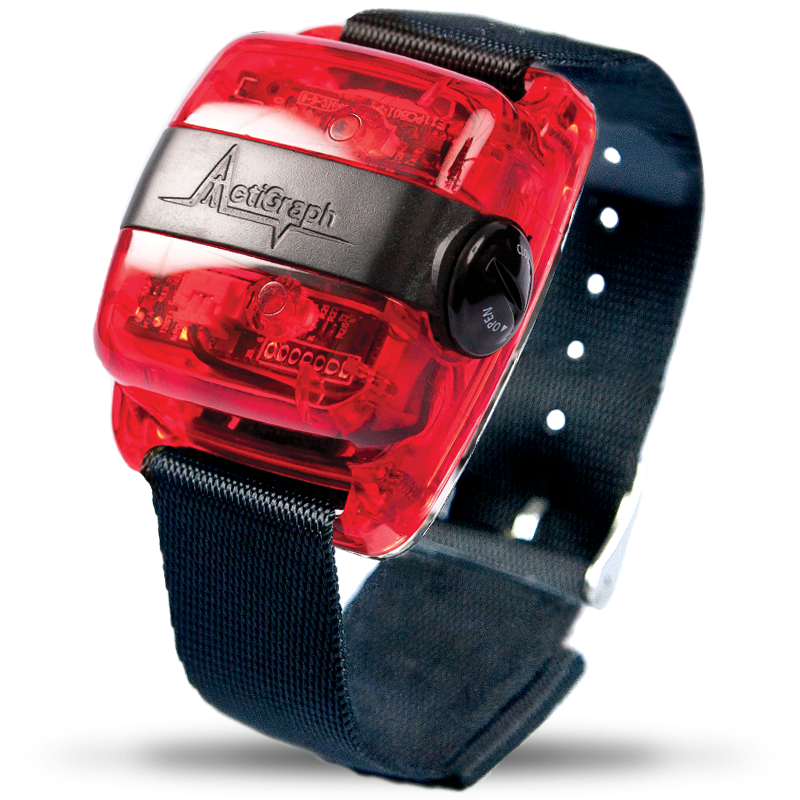
\includegraphics[scale=0.25]{figs/img_showcase_wgt3x-bt.png}
 \end{center}

 
\end{frame}

\begin{frame}{Actigraph units (source: \url{https://journals.plos.org/plosone/article/figures?id=10.1371/journal.pone.0216891})}
 
 \begin{center}
  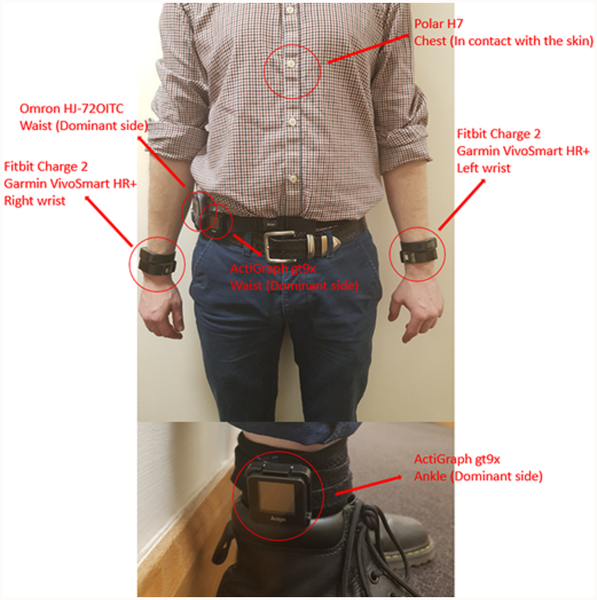
\includegraphics[scale=1.5]{figs/MultipleAccelerometers.png}
 \end{center}
 
\end{frame}

\begin{frame}{Accelerometers: (source: \url{https://www.sciencebuddies.org/science-fair-projects/references/accelerometer})}

\begin{center}
  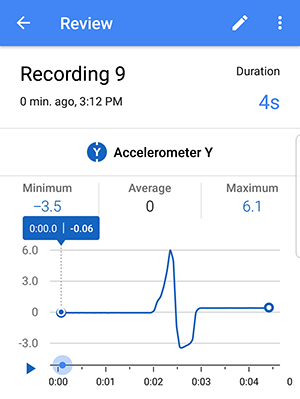
\includegraphics[scale=0.5]{figs/accel-technote-figure8-app-screenshot.png}
 \end{center}
 
\end{frame}

\begin{frame}{Accelerometers: From MAGs to METs}

{\small 
\begin{itemize}
 \item Measure acceleration along multiple axes (2 or 3).
 \[
 r(t) =
  \begin{pmatrix}
   x(t) \\ y(t) \\ z(t)
  \end{pmatrix};\quad v(t) = \frac{d}{dt}r(t);\quad a(t) = \frac{d}{dt} v(t) = \begin{pmatrix}
   \ddot{x}(t) \\ \ddot{y}(t) \\ \ddot{z}(t)
  \end{pmatrix}\;.
 \]
 
 \item Accelerometers calculate $a(t)$ over small time-intervals
 
 \item Magnitude of acceleration: $$MAG_{accel} = \sqrt{a_x^2 + a_y^2 + a_z^2},$$ where $a_x$, $a_y$ and $a_z$ are averaged accelerometer readings along the three axes over small (e.g., 10-sec) time windows (epochs).
 
 \item Metabolic Equivalent of Task (Sasaki, 2011):
 \[
  \text{MET} = 0.000863\cdot MAG + 0.668876
 \]

 \item With $MAG$ readings from hip and ankle (Mortazavi et al., 2013):
 \[
  \text{MET} = 5.289\cdot (MAG_{hip} + MAG_{ankle}) - 8.5548
 \]
\end{itemize}
}

\end{frame}

\begin{frame}{METs and MAGs by Activity Levels}
 
 \begin{table}[]
    \centering
    \begin{tabular}{l|cc}\hline
    \textbf{Activity intensity} & MET range       &  MAG \\\hline
    Sedentary or light     & $[0,\, 3)$     &   $[0,\,493)$   \\
    Moderate               & $[3,\, 6)$     &   $[493,\,1029)$     \\
    Hard                   & $[6,\, 9)$     &   $[1029,\,1608)$    \\
    Very hard              & $[9,\,\infty)$ &   $[1608,\,\infty)$     \\ \hline
    \end{tabular}
    \caption{MAG activity count cut-points for different PA intensity levels}
    \label{tab:METCutPoins}
\end{table}
 
\end{frame}


\begin{frame}{Trajectories (from GPS) carved out by subjects}
 
 \begin{center}
  \includegraphics[width=0.45\textwidth]{../../MarcoMignonePierfrancesco/images/ObservedLocationsWestwoodMap.pdf}
  \includegraphics[width=0.45\textwidth]{../../MarcoMignonePierfrancesco/images/MAGWestwoodMapFirst10PIDs.pdf}
 \end{center}
 
\end{frame}


\begin{frame}
\frametitle{Statistics and Data Science...Is Happening}

\begin{columns}[c]
\column{2.0in}

\begin{center}
Hal Varian, Google's chief economist:
\end{center}
\begin{quote}
%I keep saying the sexy job in the next ten years will be statisticians. People think I'm joking, but who would've guessed that computer engineers would've been the sexy job of the 1990s? 
The ability to take data-to be able to understand it, to process it, to extract value from it, to visualize it, to communicate it-that's going to be a hugely important skill in the next decades
\end{quote}
\vfill
\begin{quote}
{\tiny Source: \url{http://www.mckinseyquarterly.com/Hal_Varian_on_how_the_Web_challenges_managers_2286}}
\end{quote}
\column{3.0in}
\begin{center}
  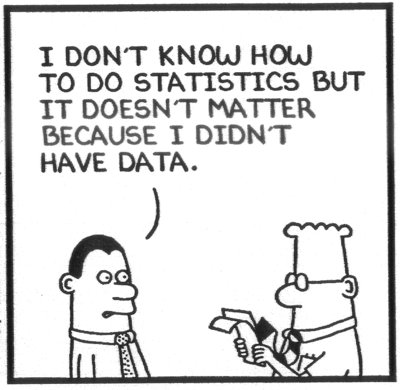
\includegraphics[width=2.0in]{figs/dilbert_statistician.jpg}\\

\end{center}

\end{columns}

\end{frame}


\begin{frame}
    \frametitle{The Information Revolution}
    \begin{itemize}\setlength{\itemsep}{0.3cm}
        \item We live in an Information Age.  \pause
        \item Computers collect and store information in quantities that were earlier unimaginable. \pause
        \item What is this information? \pause
        \begin{itemize}
            \item Measurements, counts, costs, sales revenue...
            \item arising in sciences, public health, business...
        \end{itemize} \pause
        \item Raw, ``undigested'' data stored on computer disks is useless unless we make sense of it. \pause
        \item Statistics: the art and science of extracting meaning from seemingly incomprehensible data. \pause
        \item Make good use of \emph{information} to make sound \emph{decisions}.
    \end{itemize}
\end{frame}


\begin{frame}{A favorite cartoon}

\begin{center}
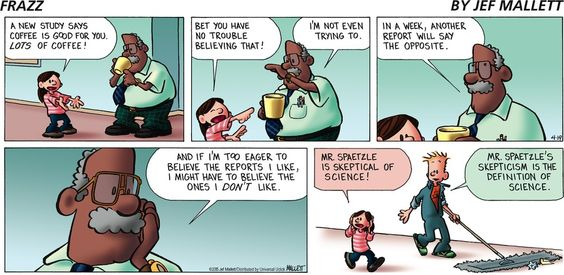
\includegraphics[height=2.5in,width=3.75in]{figs/Frazz_04_19_2015.jpg} 
\end{center}
 
\end{frame}


\begin{frame}
\frametitle{What is Statistics?}
\framesubtitle{Statistics uses math.  Statistics is not math!}
\begin{columns}[c]
\column{2.2in}

\begin{itemize}
\item Statistics: induction, inference, generalization.
\item Statistics: From data, what can we conclude about the world?
\item Mathematics: deduction.
\item Math modeling: If this model is true, what data occurs?
\item Problem: Data can occur under lots of models.  Which model is right?
\item Mathematics vital: Statistics uses math!
\end{itemize}
\column{3.5in}
%\begin{figure}
  % Requires \usepackage{graphicx}
  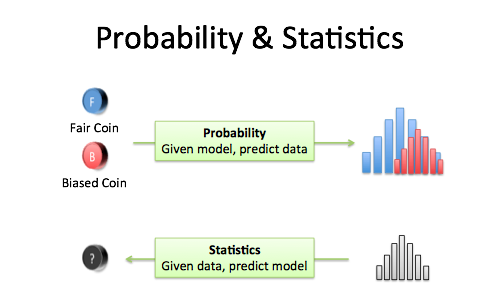
\includegraphics[width=2.5in]{figs/probability_vs_stats.png}\\
%  \caption{}\label{}
%\end{figure}
\end{columns}

\end{frame}

\begin{frame}
      \frametitle{What is Statistics?}
      \framesubtitle{Statistics applies to almost any field of science} 
      
      In one week a statistician may: \pause

       \begin{itemize}%\setlength{\itemsep}{0.3cm}
           \item help design an experiment to evaluate the effects of a new treatment for a
           disease, \pause
           \item analyze data gathered in the Amazon rain forests by an ecologist, \pause
           \item help predict how the California wild fires will
           spread, \pause
           \item help Google design a better search engine, \pause
           \item analyze data from researchers trying to find
           genes that cause breast cancer.
           \end{itemize}
 \end{frame}


\begin{frame}{Bayesian Statistical Modeling and Inference}

\[
 [\mbox{Unknown}\given \mbox{Known}] = \left[\mbox{process},\, \mbox{parameters}\given \mbox{data}\right]
\]
\begin{multline*}
 \left[\mbox{data}\given \mbox{process},\, \mbox{parameters}\right] \\ 
 \times \left[\mbox{process}\given \mbox{parameters}\right] \\
 \times \left[\mbox{parameters}\right]\;.
\end{multline*}

\begin{itemize}
 \item Process drives inference;
 \item Interpolate process at arbitrary locations;
 \item Predict scientific phenomenon (weather);
 \item Keep an eye on scalability (BIG DATA).
\end{itemize}

\end{frame} 

\begin{frame}{Estimating daily ``periodic'' behavior}
 
 \begin{center}
  \includegraphics[width=3in, height=1.5in]{../../MarcoMignonePierfrancesco/images/TsplineEstAllLinear.pdf}
  \includegraphics[width=3in, height=1.5in]{../../MarcoMignonePierfrancesco/images/TsplineEstAll.pdf}
 \end{center}

\end{frame}


\begin{frame}{Predicted METs along trajectories}
 
 \begin{center}
  \includegraphics[width=\textwidth]{../../MarcoMignonePierfrancesco/images/204_17363_MAGFixedScale_pathtogether.pdf}
 \end{center}

\end{frame}


\begin{frame}
\frametitle{Spatially Misaligned Data}
 
\begin{center}
\begin{overpic}[width=\textwidth]{../BiostatOpenHouse/dataTypes.png}
% \put(50,150){(a)}
% \put(250,150){(b)}
% \put(50,25){(c)}
% \put(250,25){(d)}
\end{overpic}
\end{center}

\end{frame}

\begin{frame}{Mapping asthma hospitalizations in California}

\begin{center}
\includegraphics[width=\textwidth, height=0.75\textheight]{../ArealModelling/Asthma_(years).png}
\end{center}

\end{frame}


\begin{frame}{Mapping asthma hospitalizations in California}

\begin{center}
\includegraphics[width=\textwidth, height=0.75\textheight]{../ArealModelling/Covariates.png}
\end{center}

\end{frame}

\begin{frame}{Mapping asthma hospitalizations in California}

{\small
\[
 \mbox{[Asthma]}_t = \mbox{[Trends]}_t + \mbox{[Explanatory]}_t + \mbox{[(Space-time) Interactions]}_t
\]
}
\vspace{-0.25cm}
\begin{center}
\includegraphics[width=\textwidth, height=0.75\textheight]{../ArealModelling/Asthma_(months).png}
\end{center}

\end{frame}

\begin{frame}{Data Analysis---Parameter Estimates}
\begin{table}[F] %t...
%\begin{singlespace}
\scriptsize
\begin{center}
\begin{tabular}{l|c||l|c}
\hline
Parameter & Median (95\% CI)  & Parameter & Median (95\% CI)\\
\hline
$\beta_{0}$ (Intercept)	&	9.51 (8.46, 10.51)	&	$\beta_{15}$ -- $\beta_{26}$ (Ozone)	&	\\		
$\beta_{1}$ (Pop Den)	&	0.63 (0.55, 0.71)	&	---\;January	&	0.51 (-0.95, 1.94)	\\
$\beta_{2}$ (\% Black)	&	1.23 (1.13, 1.33)	&	---\;February	&	0.39 (-0.61, 1.53)	\\
$\beta_{3}$ (\% $< 18$)	&	1.24 (1.13, 1.34)	&	---\;March	&	0.42 (-0.05, 0.89)	\\
$\beta_{4}$ (Feb)	&	-0.36 (-1.49, 0.85)	&	---\;April	&	0.21 (-0.05, 0.49)	\\
$\beta_{5}$ (Mar)	&	-0.24 (-1.32, 0.83)	&	---\;May	& 	-0.17 (-0.33, 0.00)	\\
$\beta_{6}$ (Apr)	&	-1.60 (-2.66, -0.51)	&	---\;June	&	-0.36 (-0.53, -0.20)	\\
$\beta_{7}$ (May)	&	-1.39 (-2.46, -0.30)	&	---\;July	&	-0.22 (-0.35, -0.09)	\\
$\beta_{8}$ (June)	&	-2.46 (-3.59, -1.37)	&	---\;August	&	-0.20 (-0.33, -0.07)	\\
$\beta_{9}$ (July)	&	-3.29 (-4.47, -2.19)	&	---\;September	&	-0.28 (-0.42, -0.12)	\\
$\beta_{10}$ (Aug)	&	-3.16 (-4.33, -2.08)	&	---\;October	&	 0.06 (-0.13, 0.25)	\\
$\beta_{11}$ (Sep)	&	-1.94 (-3.03, -0.88)	&	---\;November	&	 0.52 (0.03, 1.05)	\\
$\beta_{12}$ (Oct)	&	-1.78 (-2.82, -0.70)	&	---\;December	&	3.15 (1.43, 5.08)	\\
$\beta_{13}$ (Nov)	&	-0.87 (-1.94, 0.24)	&	Spatial smoothing	&	0.88 (0.85, 0.90)	\\
$\beta_{14}$ (Dec)	&	 2.42 (1.12, 3.64)	&	Temporal decay		&	1.24 (1.18, 1.30)	\\
\hline							
\end{tabular}
\end{center}
  \caption{Estimates and Credible Values of variables on asthma hospitalization rates.}
  \label{tab:asthma} %table updated 11/13/12
  %\end{singlespace}
\end{table}
\end{frame}
 
 \begin{frame}{Spatial-Temporal BIG DATA Analytics}

 {\tiny
\[
 \mbox{[Asthma]}_t = \mbox{[Intercept]}_t + \mbox{[Explanatory Variables]}_t + \mbox{[Space-time Interactions]}_t
\]
}

\begin{center}
\includegraphics[width=\textwidth, height=0.75\textheight]{../ArealModelling/Asthma_(overall)_tran.png}
\end{center}

\end{frame}
 

\begin{frame}
\frametitle{Spatial-Temporal BIG DATA Analytics}
\framesubtitle{To Illustrate What You Could Be Doing}{Example~1: U.S. forest biomass data}
\begin{figure}[]
\begin{center}
\vskip-4mm{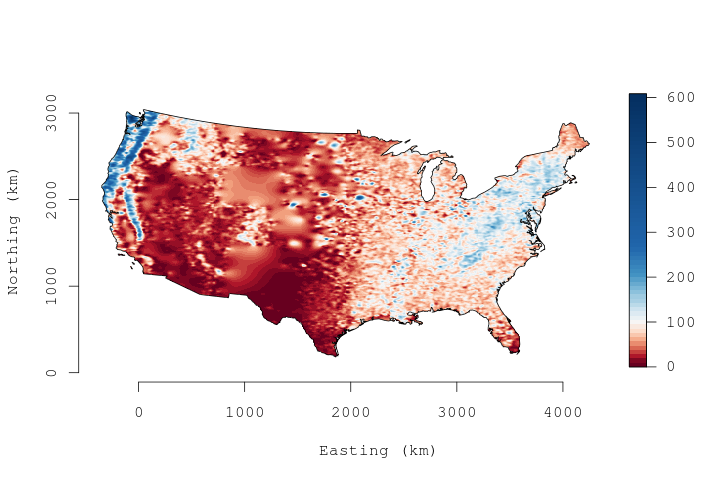
\includegraphics[width=5cm]{../Harvard_2014/figures/real/obs-biomass.png}\label{bio-obs}}
{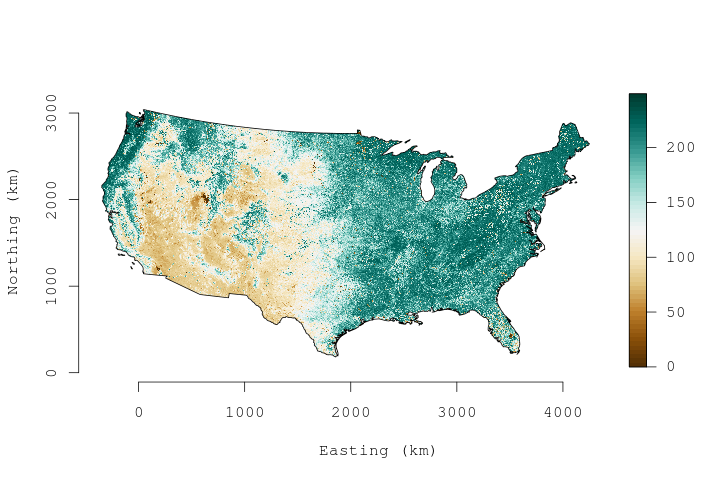
\includegraphics[width=5cm]{../Harvard_2014/figures/real/ndvi.png}\label{bio-ndvi}}
\end{center}
\caption{Observed biomass (left) and NDVI (right)}\label{fig:bio}
\end{figure}
\vspace{-0.5cm}\begin{itemize}
\item Forest biomass data collected over 114,371 plots
\item Normalized Difference Vegetation Index (NDVI) is a measure of greenness
\item {\small Forest Biomass Regression Model: $Biomass(\ell) = \beta_0(\ell) + \beta_1(\ell) NDVI(\ell) + error$}
\end{itemize}

\end{frame}


\begin{frame}
\frametitle{Spatial-Temporal BIG DATA Analytics}
\framesubtitle{Example~2: European Particulate Matter (PM$_{10}$) data}
\begin{figure}[]
\begin{center}
\vskip-8mm{\subfigure[PM$_{10}$ levels in March, 2009]{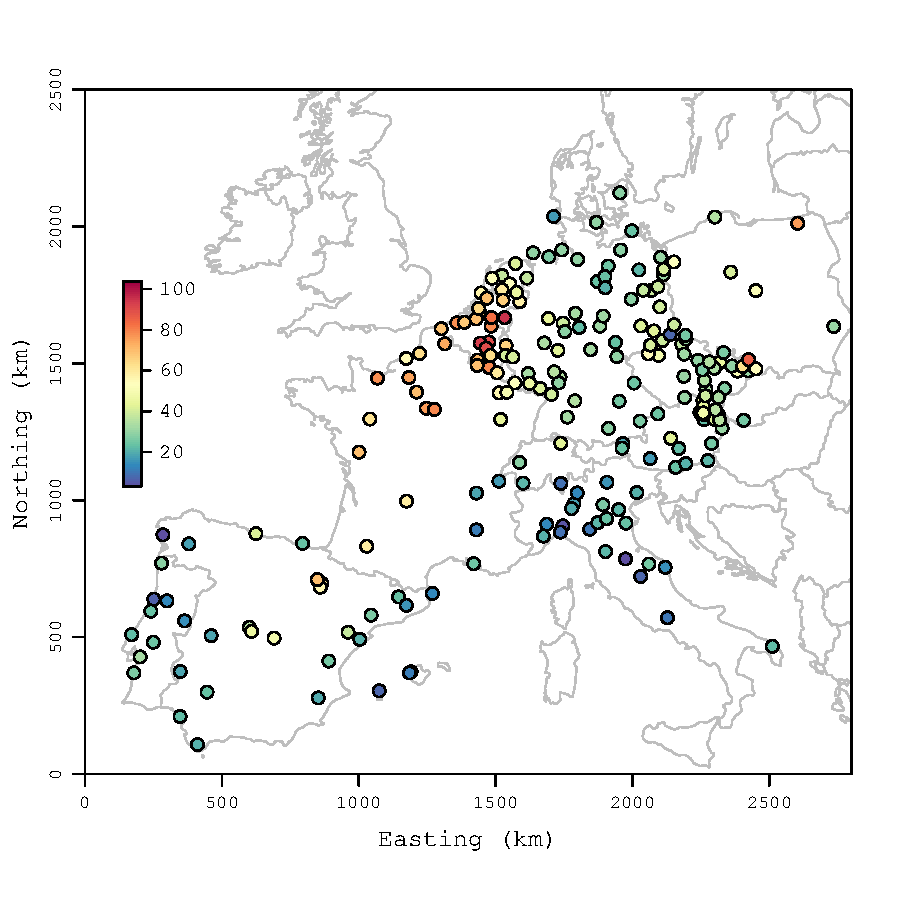
\includegraphics[width=5cm]{../Abhirup_Datta/DNNGP/figures/march-obs.pdf}\label{march-obs}}}
\subfigure[PM$_{10}$ levels in June, 2009]{{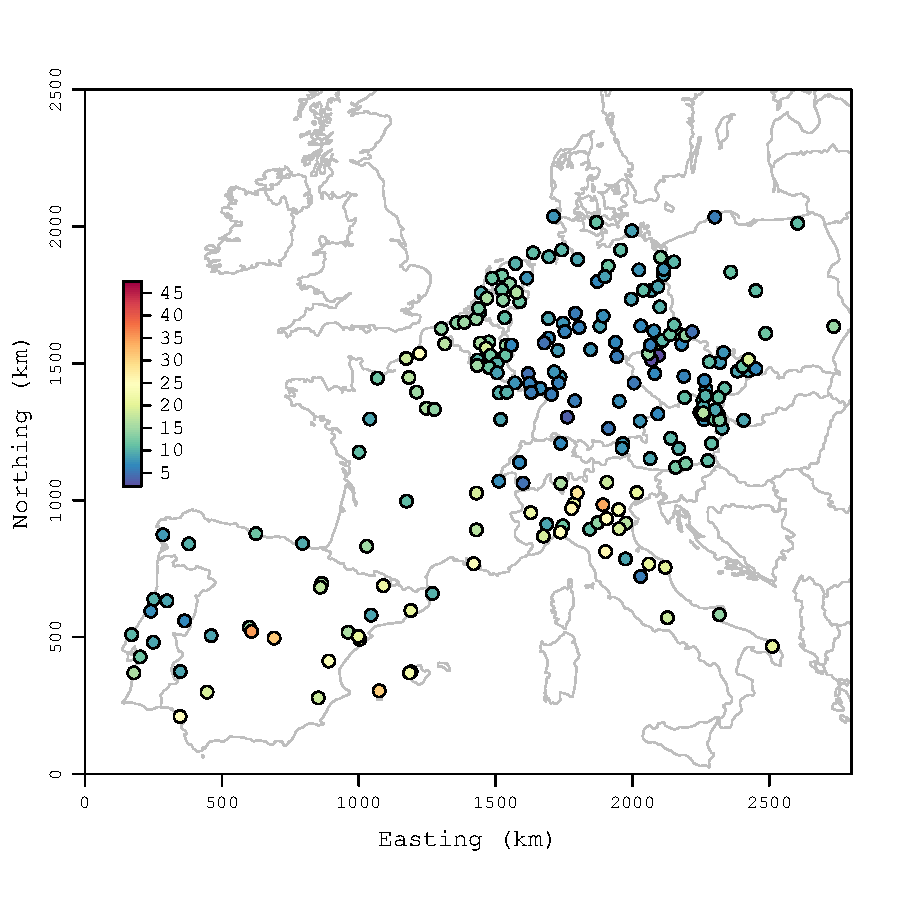
\includegraphics[width=5cm]{../Abhirup_Datta/DNNGP/figures/june-obs.pdf}\label{june-obs}}}
\end{center}
\end{figure}
\vspace{-0.5cm}
\begin{itemize}
\myitem Significant variation across space and time
\myitem Daily observations at $308$ stations for 2 years i.e., $n=308\times 730=$ \textcolor{red}{$224,840$}
\end{itemize}
\end{frame}

\begin{frame}
\frametitle{Statistical mapping with BIG DATA}
\framesubtitle{European PM$_{10}$ Dataset}
\begin{figure}
\begin{center}
\only<1>{\vskip-8mm\subfigure[$\widehat{\mbox{PM}_{10}}$ for 04.03.2009]{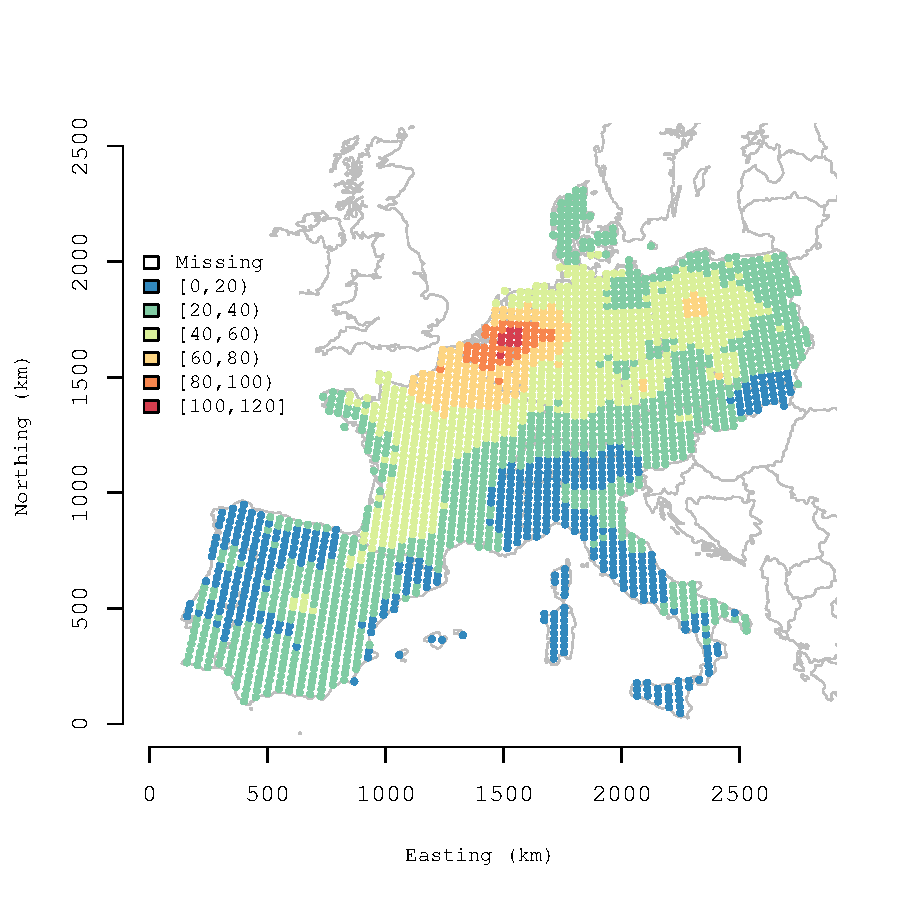
\includegraphics[width=5cm,trim={2.5cm 3cm 1cm 2cm},clip]{../Abhirup_Datta/DNNGP/figures/2009-4-3-ctm-grid-pred-mu.pdf}}
\subfigure[$Pr(\widehat{\mbox{PM}_{10}} > 50 \mu g m^{-3})$]{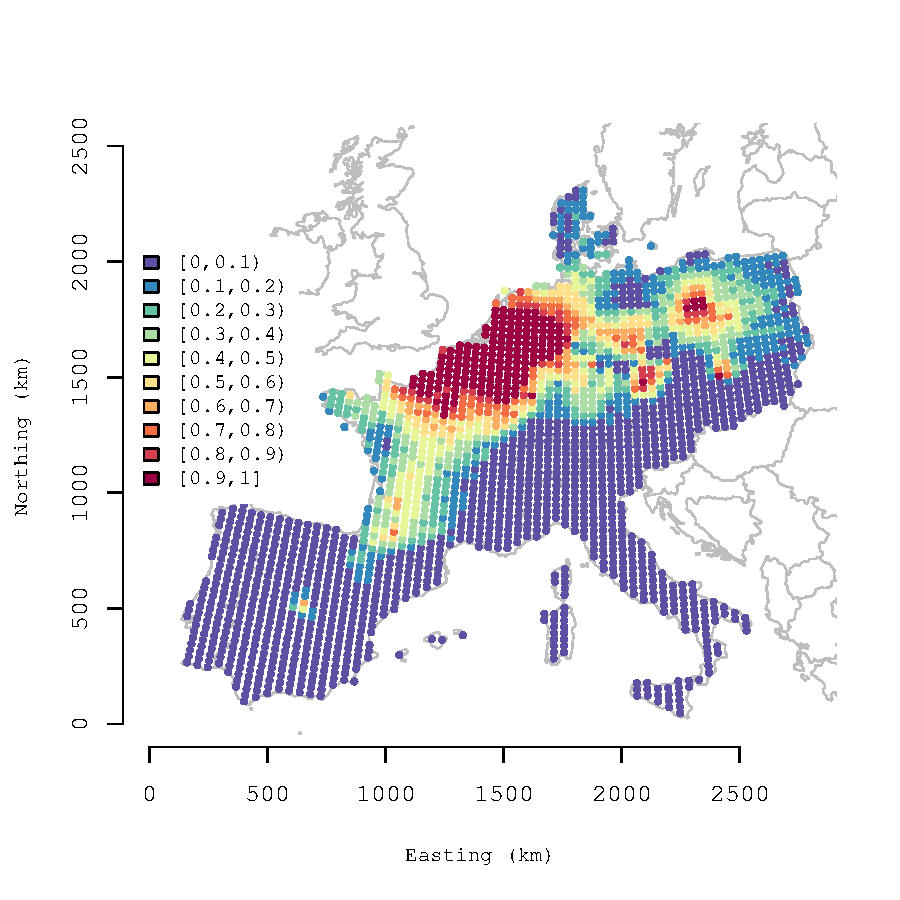
\includegraphics[width=5cm,trim={2.5cm 3cm 1cm 2cm},clip]{../Abhirup_Datta/DNNGP/figures/2009-4-3-ctm-grid-pred-prob-over-50.pdf}}}
\setcounter{subfigure}{0}
\only<2>{\vskip-8mm\subfigure[$\widehat{\mbox{PM}_{10}}$ for 04.05.2009]{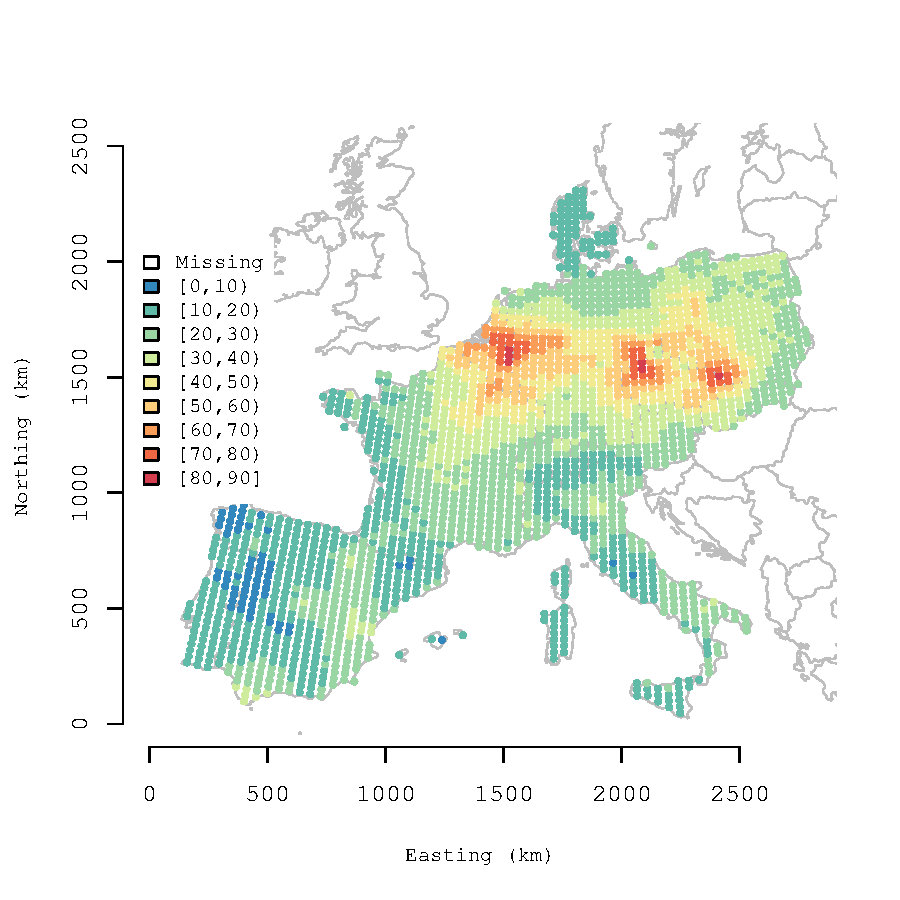
\includegraphics[width=5cm,trim={2.5cm 3cm 1cm 2cm},clip]{../Abhirup_Datta/DNNGP/figures/2009-4-5-ctm-grid-pred-mu.pdf}}
\subfigure[$Pr(\widehat{\mbox{PM}_{10}} > 50 \mu g m^{-3})$]{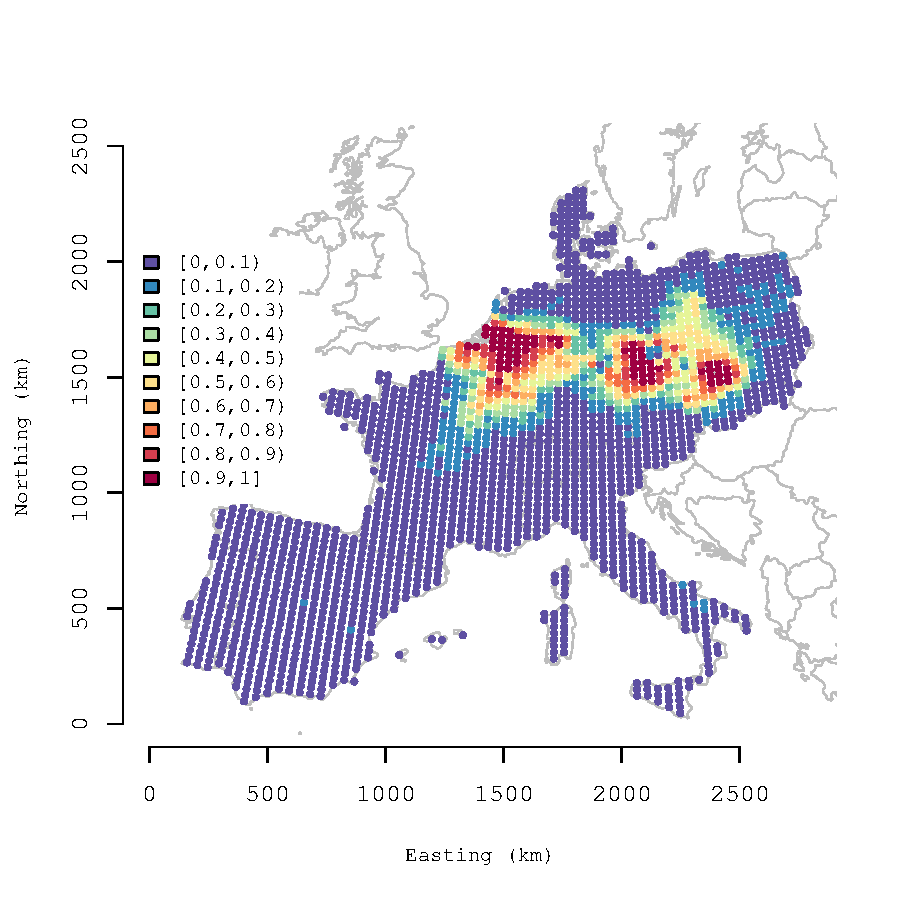
\includegraphics[width=5cm,trim={2.5cm 3cm 1cm 2cm},clip]{../Abhirup_Datta/DNNGP/figures/2009-4-5-ctm-grid-pred-prob-over-50.pdf}}}
\end{center}
%\vspace{-0.5cm}\caption{Predicted PM$_{10}$ and probability of exceeding 50 $\mu g$ $m^{-3}$ for two different dates}
\end{figure}

\end{frame}

\begin{frame}{Case Study: Tanana Valley Forest Height Analysis}
	\vskip -5mm \begin{figure}[!ht]
		\begin{center}
			\subfigure[Forest height and tree cover]{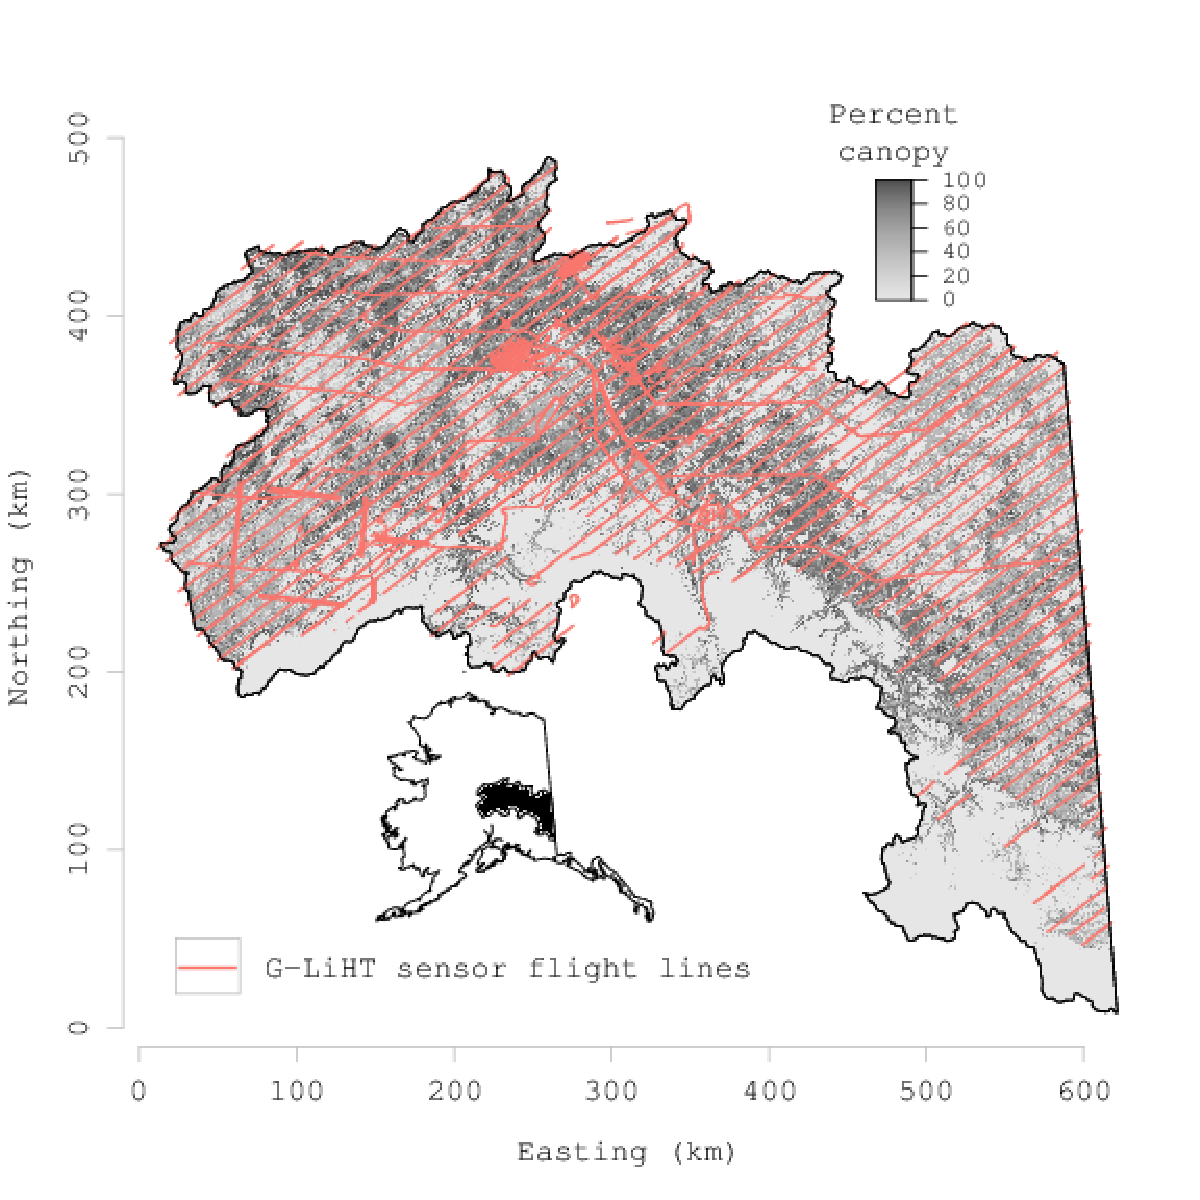
\includegraphics[width=5.3cm]{../Abhirup_Datta/spatstatJSM2017-master/figures/ak-flight-han2010.pdf}\label{han}}
			\subfigure[Forest fire history]{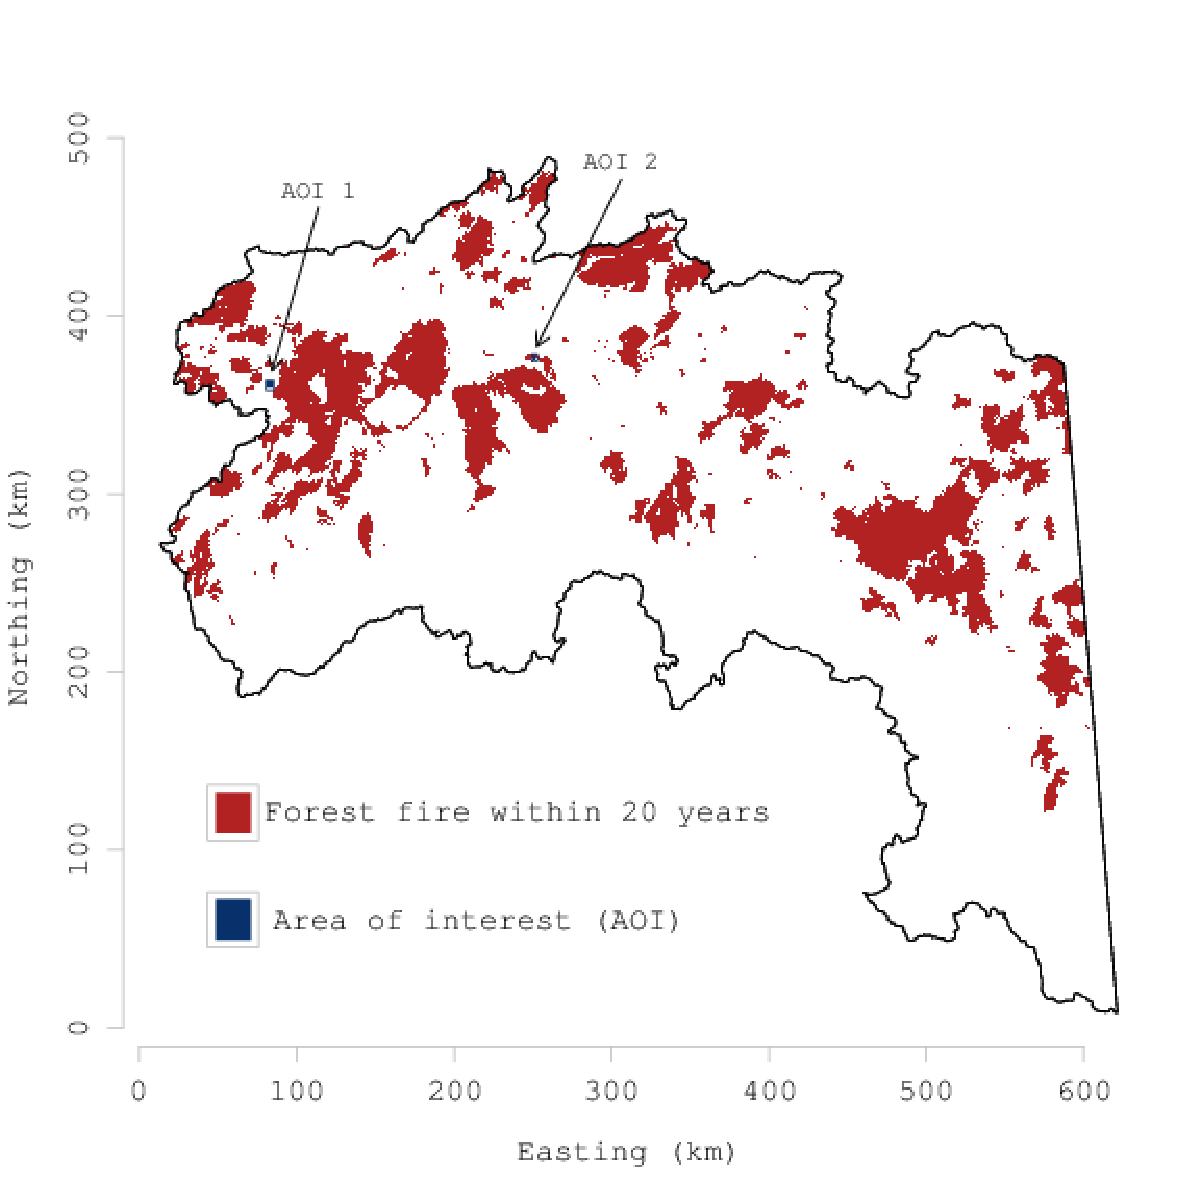
\includegraphics[width=5.3cm]{../Abhirup_Datta/spatstatJSM2017-master/figures/ak-fire.pdf}\label{fire}}
		\end{center}
		%\caption{Tanana valley, Alaska, study region. \subref{han} G-LiHT flight lines where canopy height was measured at 6x$10^6$n locations over the percent forest canopy covariate. \subref{fire} Occurrence of forest fire in the past 20 years and areas of interest for prediction illustration.}
	\end{figure}
	\vskip -4mm 
	\only<1>{{\tiny \begin{itemize}
			\item Forest height (red lines) data from LiDAR at \alert{$40\times 10^6$} locations
			\item Knowledge of forest height is important for biomass assessment, carbon management etc
	\end{itemize}}}
	\only<2>{{\tiny \begin{itemize}
			\item Goal: High-resolution domainwide prediction maps of forest height 
			 \item $\mbox{Biomass} = \mbox{[Mean]} + \mbox{[Tree Cover]} + \mbox{[Forest Fire]} + \mbox{[Spatial Process]}$ 
			\item Methodology: Entire model-based spatial data analysis done is 2 minutes on a modest laptop. 
	\end{itemize}}}
\end{frame}


\begin{frame}{Selected papers on Spatial BIG DATA analysis}

{\tiny
\begin{itemize}
 \item Banerjee, S. (2017). High-dimensional Bayesian geostatistics. \emph{Bayesian Analysis}, 12, 583--614. DOI: \url{http://dx.doi.org/10.1214/17-BA1056R}

 \item Banerjee, S. (2020). Modeling massive spatial datasets using a conjugate Bayesian linear modeling framework. \emph{Spatial Statistics}, 37, 10047. DOI: \url{https://doi.org/10.1016/j.spasta.2020.100417}
 
 \item Banerjee, S., Gelfand, A.E., Finley, A.O. and Sang, H. (2008). Gaussian predictive process models for large spatial datasets. \emph{Journal of the Royal Statistical Society Series B}, 70, 825--848. DOI: \url{http://dx.doi.org/10.1111/j.1467-9868.2008.00663.x}
 
 \item Datta, A., Banerjee, S., Finley, A. O., and Gelfand, A. E. (2016).  Hierarchical Nearest-Neighbor Gaussian Process models for large geostatistical datasets. \emph{Journal of the American Statistical Association}, 111, 800--812. DOI: \url{http://dx.doi.org/10.1080/01621459.2015.1044091}

 \item Datta, A., Banerjee, S., Finley, A. O., Hamm, N. A. S., and Schaap, M. (2016). Non-separable dynamic Nearest-Neighbor Gaussian Process models for large spatio-temporal data with an application to particulate matter analysis. \emph{Annals of Applied Statistics}, 10, 1286--1316. DOI: \url{http://dx.doi.org/10.1214/16-AOAS931}  
 
 \item Finley, A. O., Datta, A., Cook, B. C., Morton, D. C., Andersen, H. E., and Banerjee, S. (2019). Applying Nearest Neighbor Gaussian Processes to massive spatial data sets: Forest canopy height prediction across Tanana Valley Alaska. \emph{Journal of Computational and Graphical Statistics}. DOI: \url{https://doi.org/10.1080/10618600.2018.1537924}
 
 \item Guinness, J. (2018). Permutation methods for sharpening Gaussian Process approximations. \emph{Technometrics}, 60, 415--429.
 
 \item Heaton, M., Datta, A., Finley, A., Furrer, R., Guhaniyogi, R., Gerber, F., Hammerling, D., Katzfuss, M., Lindgren, F., Nychka, D., and Zammit-Mangion, A. (2017). Methods for analyzing large spatial data: A review and comparison. \emph{arXiv:1710.05013}.

\item Katzfuss, M. (2017). A multi-resolution approximation for massive spatial datasets. \emph{Journal of the American Statistical Association}, 112, 201--214.
 
\item Katzfuss, M. and Guinness, J. (2017). A general framework for vecchia approximations of gaussian processes. \emph{arXiv preprint arXiv:1708.06302}.

\item Nychka, D., Bandyopadhyay, S., Hammerling, D., Lindgren, F., and Sain, S. (2015). A multiresolution gaussian process model for the analysis of large spatial datasets. \emph{Journal of Computational and Graphical Statistics}, 24, 579--599. 
 
% \item Nychka, D., Wikle, C., and Royle, J. A. (2002). Multiresolution models for nonstationary spatial covariance functions. \emph{Statistical Modelling}, 2, 315--331.

\item Peruzzi, M., Banerjee, S. and Finley, A.O. (in press). Highly scalable Bayesian geostatistical modeling via meshed Gaussian processes on partitioned domains. \emph{Journal of the American Statistical Association}, DOI: \url{https://doi.org/10.1080/01621459.2020.1833889}. 
 
\item Taylor-Rodriguez, D., Finley, A.O., Datta, A., Babcock, C., Andersen, H.E., Cook, B.C., Morton, D.C. and Banerjee, S. (2019).  Spatial factor models for high-dimensional and large spatial data: An application in forest variable mapping. \emph{Statistica Sinica}, {29}, 1155--1180. DOI: \url{https://doi.org/10.5705/ss.202018.0005}.
 
 \item Zhang, L., Datta, A. and Banerjee, S. (2019). Practical Bayesian modeling and inference for massive spatial datasets on modest computing environments. \emph{Statistical Analysis and Data Mining: The ASA Data Science Journal}, {12}, 197--209. DOI: \url{https://doi.org/10.1002/sam.11413}
\end{itemize}
}
 
\end{frame}

\begin{frame}
 
 \begin{center}
  {\Huge Thank You!}
 \end{center}

\end{frame}

\end{document}




